\chapter{Non imaging optics}
This chapter provides the notions of illumination optics needed in this thesis. We start expaining the difference between radiometry and photometry.
We define the photometric variables  both in three and two dimensions. The reflection and refraction laws and the phenomenon of total internal reflection are explained. The last paragraph of the chapter gives a brief introduction of the Fresnel's equations. 
\section{Radiometric and photometric variables}
Radiometry is the measurement of the electromagnetic radiation across the entire electromagnetic spectrum. Photometry is the subfield of radiometry that takes into account only the portion of the electromagnetic spectrum corresponding to the visible light, \cite{zalewski1995radiometry}. Radiometry  deals with radiometric quantities. An important radiometric quantity  is the radiant flux $\Phi_{\textrm{r}}$ (unit watt, [\textrm{W}]) which is the total energy emitted from a source or received by a target per unit time:
\begin{equation}
\Phi_{\textrm{r}} = \frac{\textrm{d}Q}{\textrm{d}T}\,,
\end{equation}
where $Q$ is the energy and $T$ the time.\\
\indent In Illumination optics the measurement of light is given in terms of the impression that it gives on the human eyes. Therefore, illumination optics deals with the photometric variables. The most important photometric variables are defined as in the following. The luminous flux $\Phi$ (unit lumen, [\textrm{lm}]) is defined as the perceived power of light by the human eye, \cite{chaves2015introduction}.
 The radiant and the luminous flux are related by the luminous efficacy function, unit [lm/W], that tells us how many lumen there are for each Watt of power at a given wavelength.
 The luminous efficacy reaches its maximum  at a wavelength of $555$ $\textrm{nm}$ where it is equal to $683$ $\textrm{lm}/\textrm{W}$.
  We may normalize the luminous efficacy function with its maximum value of $683$.
  This normalized function is the dimensionless luminosity function $\bar{y}(\lambda)$ shown in Figure $\ref{fig:luminosityfunction}$ where $\lambda$ is the wavelength.
\begin{figure}[htbp]
%\label{fig:luminousfunction}
  \begin{center}
  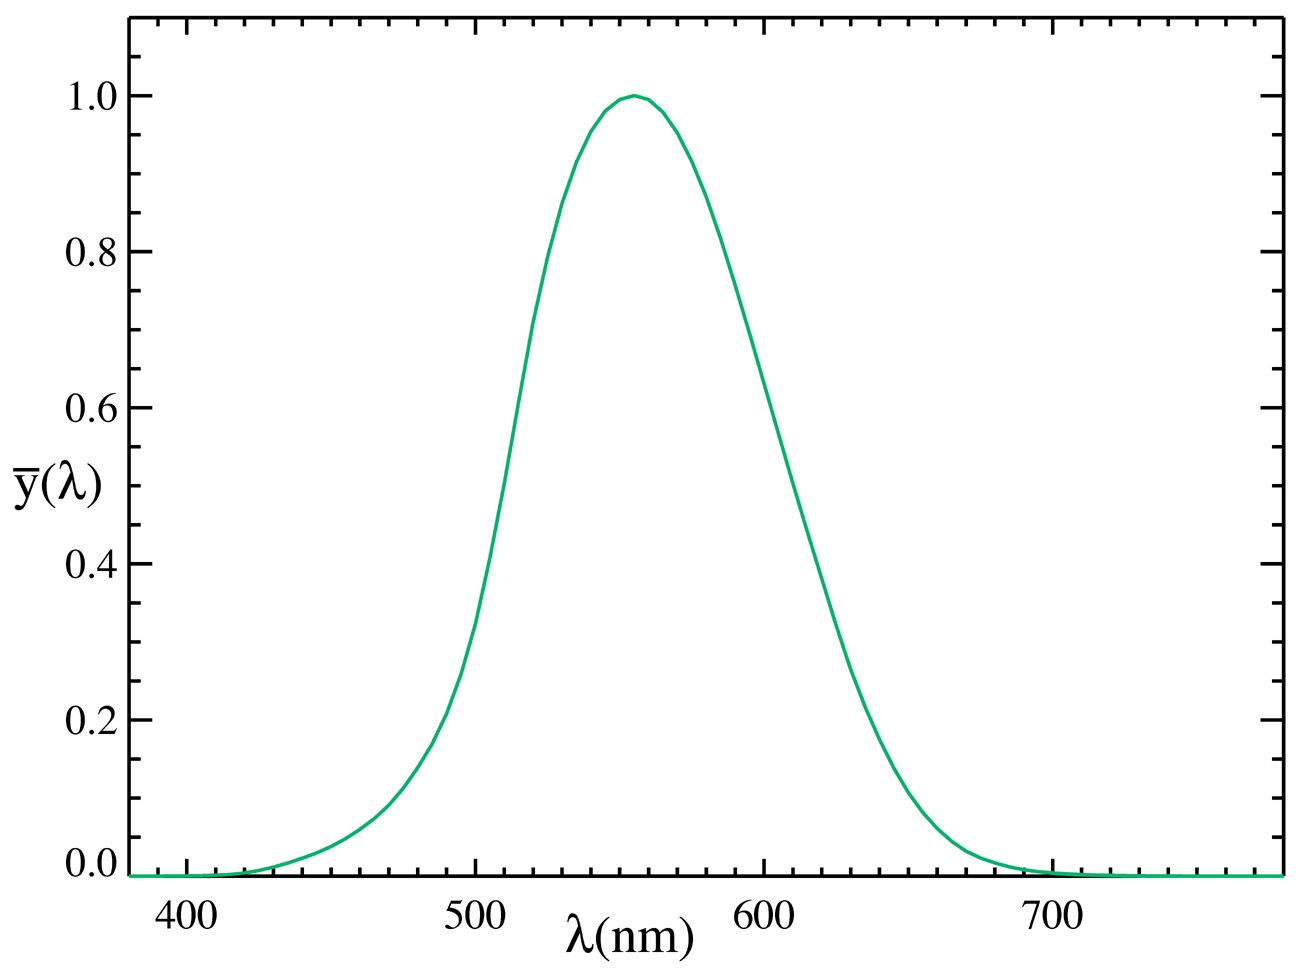
\includegraphics[width=7cm]{CIELuminosity}
  \end{center}
  \caption{Luminosity function $\bar{y}(\lambda)$: relation between the eye's sensitivity and the wavelength of the light. The luminous function is dimensionless.}
  \label{fig:luminosityfunction}
  \end{figure}
\\ The luminous flux corresponding to one Watt of radiation power at any wavelength is given by the product of $683$ $\textrm{lm/W}$ and the luminosity function at the same wavelength,
i.e. $683 \, \bar{y}(\lambda)$. Hence, $\Phi$ has unit lumen [\textrm{lm}] and it is defined as:
\begin{equation}
\Phi = 683 \int_0^\infty \Phi_\textrm{r}(\lambda) \bar{y}(\lambda)\textrm{d}\lambda \;.
\end{equation}
\indent The luminous flux $\textrm{d}\Phi$ falling on a surface is called illuminance $E$ \big(unit \big[$\textrm{lm}/\textrm{m}^2\big]$\big)
and is defined as:
\begin{equation}
 E=\frac{\textrm{d}\Phi}{\textrm{d}A}\;,
 \end{equation}
 where $\textrm{d}A$ is an infinitesimal area receiving energy. The solid angle describes the angular density of light emitted by a point source. The solid angle subtended by the light is defined by the surface area of a sphere subtended by the radius of that sphere and by the rays emitted by the point source where a light ray can be defined as a path along which the energy travels.The solid angle is indicated with $\Omega$ and the dimensionless unit of solid angles is the steradian $[sr]$, \cite{arecchi2007field}. Indicating with $r$ the radius of the sphere, the infinitesimal solid angle $\textrm{d}\Omega$ defined by the infinitesimal surface $\textrm{d}A^*$ is given by:
\begin{equation}\label{solid_angle}
\textrm{d}\Omega = \frac{\textrm{d}A^*}{r^2} 
\end{equation}
The luminous intensity $I$ (unit candela (\textrm{cd}), $[\textrm{cd}=\textrm{lm}/\textrm{sr}]$) is defined as the luminous flux $\textrm{d}\Phi$ per solid angle
$\textrm{d}\Omega$ and is given by:
\begin{equation}\label{intensity}
I = \frac{\textrm{d}\Phi}{\textrm{d}\Omega}\;.
\end{equation}
 \begin{figure}[htbp]
%\label{fig:cup}
  \begin{center}
  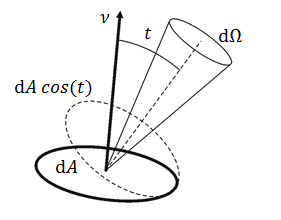
\includegraphics[width=6 cm]{immagine}
  \end{center}
  \caption{Radiation emitted in a solid angle $\textrm{d}\Omega$ in a direction making an angle $t$ with the normal to the area $\textrm{d}A$.}
  \label{fig:rad}
  \end{figure}
The luminance $L$ \big(unit $\big[\textrm{cd} / \textrm{m}^2\big]$\big) is the luminous flux per unit solid angle $\textrm{d}\Omega$ and  per unit projected area $\cos(t)\,\textrm{d}A$ that is the projection of the area element $\textrm{d}A$ on a line perpendicular to the ray.  $L$  is given by:
\begin{equation}\label{luminance1}
  L=\frac{\textrm{d}\Phi}{\cos t\textrm{d}A\textrm{d}\Omega}\;,
\end{equation}
where $t$ is the angle that the normal $\boldsymbol{\nu}$ to area $\textrm{d}A$ makes with the direction of the solid angle $\textrm{d}\Omega$, as shown in Figure $\ref{fig:rad}$.
\noindent Note that from ($\ref{intensity}$) and ($\ref{luminance1}$) we can derive a relation between the intensity and the luminance.\\
The infinitesimal intensity $\textrm{d}I $ emitted by the area element $\textrm{d}A$ is given by:
\begin{equation}
\textrm{d}I = \frac{\textrm{d}\Phi}{\textrm{d}\Omega}= L(\textrm{x},t)\cos(t)\textrm{d}A \,.
\end{equation}
When the luminance is uniform over a finite area $A$, the luminous intensity emitted in the direction $t$ is equal to:
\begin{equation}
I(t) = L(\variabile{t}) A \cos(t)\,.
\end{equation}
Thus, when $L(\textrm{x},t)$ does not depend on the position and the direction (i.e. $L(\textrm{x},t)=L$), we deduce Lambert's cosine law:
\begin{equation}
I(t) = I_0\cos(t)\,.
\end{equation}
where $I_0 = I(0) = LA$. \\
Finally the \'{e}tendue $U$ (unit $[m \cdot srad]$) describes the ability of a source to emitt light or the capability of an optical system to receive light, \cite{zhu2011etendue}.
The quantity $ \textrm{d}U $ is defined as:
\begin{equation}\label{etendue}
\textrm{d}U = n^2 \cos(t) \textrm{d}A\textrm{d}\Omega.
\end{equation}
where $n$ is the index of refraction of the medium in which the infinitesimal surface $A$ is immersed. In optics the \'{e}tendue is considered to be a volume in phase space  (or an area for two-dimensional systems). This concept will be clarified in Chapter \ref{chap:PS} where we treat the phase space in more details.
An important property of the \'{e}tendue is that it is conserved in an optical system where the flux is constant. In the following we show how the conservation of this quantity can be derived following the same approched used by J. Chaves in \cite{chaves2015introduction}.
Consider a light ray emitted from an infinitesimal area $\textrm{d}A_1$ in the direction of  $\textrm{d}A_2$,  see Figure \ref{fig:etendue_conservation}.
\begin{figure}[htbp]
 \label{fig:etendue_conservation}
     \begin{center}
     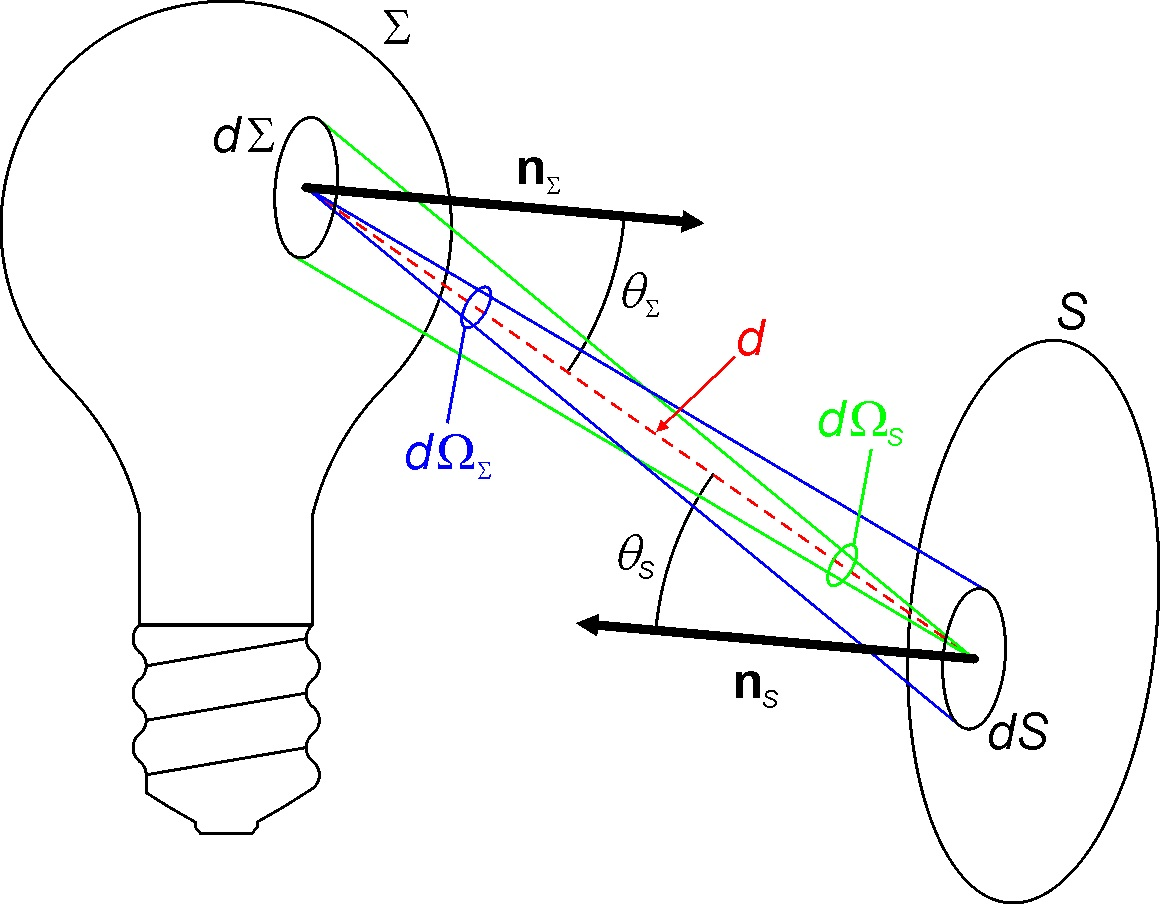
\includegraphics[width=10cm]{Etendue-Free_space.jpg}
     \end{center}
     \caption{\footnotesize{$\textrm{d}A_1$ and $\textrm{d}A_2$ are two line surfaces with normal $\nu_1$ and $\nu_2$, respectively. $t_1$ and $t_2$ are the angles made by the central ray with the normals $\nu_1$ and $\nu_2$, respectively.}}
\label{fig:etendue_conservation}
 \end{figure}
The two areas $\textrm{d}A_1$ and $\textrm{d}A_2$ are located at a distance $d$. The flux passing though $\textrm{d}A_2$ coming from $\textrm{d}A_1$ is equal to:
\begin{equation}
\textrm{d}\Phi_1 = L \cos(t_1) \textrm{d}A_1 \textrm{d}\Omega_1
\end{equation}
with $\textrm{d}\Omega_1$ defined at the area $\textrm{d}A_1$ by the area $\textrm{d}A_2$ and is given by 
\begin{equation}
\textrm{d}\Omega_1 = \frac{\textrm{d}A_2\cos(t_2)}{d^2}\,.
\end{equation}
Similarly, the flux passing though $\textrm{d}A_1$ coming from $\textrm{d}A_2$ is equal to:
\begin{equation}
\textrm{d}\Phi_2 = L \cos(t_2) \textrm{d}A_2 \textrm{d}\Omega_2
\end{equation}
and
\begin{equation}
\textrm{d}\Omega_2 = \frac{\textrm{d}A_1\cos(t_1)}{d^2}\,.
\end{equation}
Then \begin{equation}
\label{etendue1}
\textrm{d}U_1 = n^2 \textrm{d}A_1\cos(t_1)\textrm{d}\Omega_1= \frac{n^2 \textrm{d}A_1\cos(t_1)\textrm{d}A_2\cos(t_2)}{d^2},
\end{equation}
and
\begin{equation}
\label{etendue2}
\textrm{d}U_2 = n^2 \textrm{d}A_2\cos(t_2)\textrm{d}t_2= \frac{ n^2 \textrm{d}A_2\cos(t_2)\textrm{d}A_1\cos(t_2)}{d^2}\,.
\end{equation}
From equation ($\ref{etendue1}$) and ($\ref{etendue2}$) we see that $\textrm{d}U_1=\textrm{d}U_2$.
For a light beam, all the light passing through $\textrm{d}A_1$ coincides with the light passing through $\textrm{d}A_2$, hence $\textrm{d}U = \textrm{d}U_1$. Moreover, for the same light beam, all the light passing from $\textrm{d}A_2$ corresponds to the light emitted from $\textrm{d}A_1$, then $\textrm{d}U=\textrm{d}U_2$. Finally we can conclude that the \'{e}tendue $\textrm{d}U$ is conserved along a beam of light. Since also the flux through the areas $\textrm{d}A_1$ and $\textrm{d}A_2$ is conserved, the following relation holds:
\begin{equation}\label{basicluminance}
L := n \frac{\textrm{d}\Phi}{\textrm{d}U} = constant\,.
\end{equation}
 In the optical systems we will consider in this work, the source and the target are located in the same medium (air) with $n=1$, so the luminance $L$ equals the basic luminance $L^* = L/n$ at the source and the target of the system.\\
\indent In this thesis we consider two-dimensional optical systems. 
 Hence, we need to find two-dimensional analogies for the definitions given above.
In two dimensions the illuminance \big(unit $\big[\textrm{lm}/\textrm{m}\big]$\big) denotes the luminous flux falling on a line segment $\textrm{d}x$ and is given by:
 \begin{equation}
 E=\frac{\textrm{d}\Phi}{\textrm{d}x}\;.
 \end{equation}
 The luminous intensity \big(unit $\big[\textrm{lm}/\textrm{rad}\big]$\big) is the luminous flux per angle $\textrm{d}t$:
 \begin{equation}
 I=\frac{\textrm{d}\Phi}{\textrm{d}t}\;.
 \end{equation}
 Thus the following relation holds:
 \begin{equation}
 \textrm{d}I = L\cos(t)\textrm{d}x\,.
 \end{equation}
 The luminance \big(unit $\big[\textrm{lm}/(\textrm{rad}\; \textrm{m})\big]$\big) is given by:
 \begin{equation}
 L = \frac{\textrm {d}^2 \Phi}{\cos t\,\textrm{d}x \,\textrm{d}t}.
 \end{equation}
 \indent The \'{e}tendue $\textrm{d}U $ (unit $[m\cdot rad]$) in $2$D is given by:
\begin{equation}\label{etendue2d}
\textrm{d}U = n\cos(t) \textrm{d}a\textrm{d}\variabile{t}
\end{equation}
where $\textrm{d}a$ is the infinitesimal length of a segment.
\section{Reflection and refraction law}
The propagation of a light ray traveling through  different media is described by the reflection and refraction law.
In this section we introduce these two laws and we explain the total internal reflection phenomenon.
A light ray is described by a position vector \vect{x} and a direction vector \vect{t} and can be parameterized by the arc length \variabile{s}.
Light rays travel in an homogeneous medium along straight lines, once they hit a reflective surface their direction changes.
 Denoting with $\vect{t}_1$ the direction of the incident ray and with $\boldsymbol{\nu}$ the unit normal to the surface at the location of the incidence, the direction $\vect{t}_2$ of the reflected ray is given by:
 \begin{equation}\label{Reflection}
  \vect{t}_2 = \vect{t}_1-2(\vect{t}_1,\boldsymbol{\nu})\boldsymbol{\nu}\,,
\end{equation}
where the vectors $\vect{t}_1$ and $\boldsymbol{\nu}$ are unit vectors. 
From Eq. (\ref{Reflection}) it follows that the vector  $\vect{t}_2$ is a unit vector too, indeed considering the scalar product $(\vect{t}_2,\vect{t}_1)$ it holds:
\begin{equation}\label{unit_vector}
(\vect{t}_2,\vect{t}_1) = (\vect{t}_1,\vect{t}_1) - 4(\vect{t}_1,\boldsymbol{\nu})(\vect{t}_1,\boldsymbol{\nu})+
4(\vect{t}_1,\boldsymbol{\nu})^2(\boldsymbol{\nu},\boldsymbol{\nu})=1 .
\end{equation} 
Denoting the incident angle with $\alpha_{\textrm{i}}$ and the reflective angle with $\alpha_\textrm{r}$ such that
\begin{equation}
\cos{\alpha_{\textrm{i}}} = -\vect{t}_1\cdot \boldsymbol{\nu} \qquad \mbox{and} \qquad \cos{\alpha_{\textrm{r}}} = \vect{t}_2 \cdot\boldsymbol{\nu}\,,
\end{equation}
the reflection law states that $\alpha_\textrm{i}$ equals $\alpha_\textrm{r}$ which are measured counterclockwise with respect to the normal $\boldsymbol{\nu}$ of the surface, see Fig. \ref{Snell}.
When a ray propagates through two media with two different indices of refraction, $n_1$ and $n_2$, the direction of the refractive ray is given by:
\begin{equation}\label{Refraction}
\vect{t}_2 = n_{1,2}\,\vect{t}_1+
\Big[\sqrt{1-n_{1,2}^2+n_{1,2}^2(\boldsymbol{\nu},\vect{t}_1)^2}-n_{1,2}(\boldsymbol{\nu},\vect{t}_1) \Big]\boldsymbol{\nu}\,,
\end{equation}
where $n_{1,2}=n_1/n_2$. \\
 \indent Note that in Eq. (\ref{Reflection}) the direction of the normal $\boldsymbol{\nu}$ to the surface is not relevant for the computation of the direction of the reflective ray, since:
\begin{equation}
\vect{t}_2 = \vect{t}_1-2(\vect{t}_1,\boldsymbol{\nu})\boldsymbol{\nu}= \vect{t}_1-2(\vect{t}_1,-\boldsymbol{\nu})(-\boldsymbol{\nu}) ,
\end{equation}
while this is not the case of Eq. (\ref{Refraction}), therefore in the latter case we need to specify the direction of the vector $\boldsymbol{\nu}$ which is chosen in such a way that the angle that it forms with the incident ray $\vect{t}_1$ is smaller than or equal to $\pi/2$. Hence, if $(\vect{t}_1, \boldsymbol{\nu})\geq0$ the normal $\boldsymbol{\nu}$ directed inside the same medium in which travels the incident ray is taken, otherwise the normal $-\boldsymbol{\nu}$ directed inside the same medium in which the transmitted ray will travel has to be considered. \\ \indent
Eq. (\ref{Refraction}) is only valid for 
\begin{equation}\label{tir}\begin{split}
1-n_{1,2}^2+n_{1,2}^2(\boldsymbol{\nu},\vect{t}_1)^2\geq 0 & \Rightarrow \frac{n_2}{n_1}\geq \sqrt{1-(\boldsymbol{\nu},\vect{t}_1)^2}\\
\Rightarrow n_2\geq n_1\sqrt{1-\cos^2(\alpha_\textrm{i})} & \Rightarrow  n_2\geq n_1 \sin(\alpha_\textrm{i})
\end{split}
\end{equation}
\\ \indent
 The angle for which the equality holds is
\begin{equation}\label{critical}
\alpha_{\textrm{c}} = \arcsin\Big(\frac{n_2}{n_1}\Big)
\end{equation} and it is called the critical angle, \cite{chaves2015introduction}.
Note that the condition $\frac{n_2}{n_1}<1$ is verified as in this case $\sin(\alpha_\textrm{i})<1$.
When the incident angle $\alpha_{\textrm{i}}$ is exactly equal to the critical angle $\alpha_{\textrm{c}}$ the refractive ray propagates parallel to the refractive surface, 
when $\alpha_{\textrm{i}}>\alpha_{\textrm{c}}$ the light ray is no longer refracted but it is reflected by the surface. This phenomenon is called total internal reflection (TIR). When there is TIR the $100\%$ of light is reflected and there is no loss of energy. Therefore, optical systems designed such that TIR occurs are very efficient. While light that hits a normal refractive mirror can be both reflected and refracted. Therefore, some part of the energy is transmitted and some part is reflected. The percentual of light that is reflected and refracted is determined by the Fresnel's coefficients.
In the next paragraph an overview of the Fresnel equations is given.

\section{The Fresnel equations}
It is useful to describe light propagation from the perspective of Electromagnetic Theory which gives information about the incident, reflected and transmitted radiant flux density that are denoted with $I_i$, $I_r$ and $I_t$, respectively. \\
In the following we make use of the same notation adopted in \cite{hecht1998hecht}, Chapter $4$.
Define the electric filed\\
Picture
 \begin{equation}
I = \frac{c\varepsilon_0}{2}E_0^2
\end{equation} where $c$ is the speed of light in vacuum, $\varepsilon_0$ is the permeability in the vacuum.\\
The incident, reflected and transmitted power are $I_i A \cos(\variabile{t}_i)$, $I_r A \cos(\variabile{t}_r)$ and $I_t A \cos(\variabile{t}_t)$, respectively.
The reflectance $R$ is the ratio of the reflected power to the incident power:
\begin{equation}\label{reflectance}
R = \frac{I_r A \cos(\variabile{t}_r)}{I_i A \cos(\variabile{t}_t)} = \frac{I_r}{I_i}
\end{equation}
Similarly, the transmittance $T$ is the ratio between the ratio of the transmitted to the incident power:
\begin{equation}\label{transmittance}
T = \frac{I_t A \cos(\variabile{t}_t)}{I_i A \cos(\variabile{t}_i)} .
\end{equation}\\
Note that 
\begin{equation}\label{R}
R = \Big(\frac{E_{0 r}}{E_{0 i}}\Big)^2
\end{equation}
since $ I_r/I_t = (v_r\varepsilon_r E_{0r}^2/2)/(v_i\varepsilon_i E_{0i}^2/2)$, 
while: \begin{equation}\label{T}
T = \frac{n_t \cos(t_t)}{n_t \cos(t_i)}\Big(\frac{E_{0 t}}{E_{0 i}}\Big)^2
\end{equation}
where we assumed that $\mu_i = \mu_t  = \mu_0$ and we used the fact that $\mu_0 v_t\varepsilon_t=n_t/c$.
The values $r = \Big(\frac{E_{0 i}}{E_{0 i}}\Big)$ and $t = \Big(\frac{E_{0 t}}{E_{0 i}}\Big)$ are called the amplitude coefficients.  
The intensity of the reflected and transmitted light depends not only on the angle of incident but also on the direction of the electric field \vect{E}, 
\cite{feynman1964feynman}.
It is necessary to derive separately the parallel and perpendicular components of $r$ and $t$. 
To do that, the Maxwell equations need to be considered. 
Then the boundaries condition that guarantees that the electric field \vect{E} tangent to the interface is continuous across it is imposed. 
After some calculations the Fresnel equations are derived for the cases of the electric field both perpendicular and parallel to the plane of incident, (see  \cite{born2013principles, hecht1998hecht} for more details). In case \vect{E} is perpendicular to the plane of incidence the following equations are obtained:
\begin{equation} \label{Fresnel_perpendicular}
\begin{split}
r_{s} & = \frac{n_i\cos(t_i)-n_t \cos(t_t)}{n_i \cos(t_i)+n_t\cos(t_t)}\\
t_{s} & =  \frac{2n_i\cos(t_i)}{n_i\cos(t_i)+n_t\cos(t_t)}
\end{split}
\end{equation}
In case \vect{E} is parallel to the plane of incidence the amplitude coefficients are:
\begin{equation}\label{Fresnel_parallel}
\begin{split}
r_{p} & = \frac{n_t\cos(t_i)-n_i \cos(t_t)}{n_i \cos(t_t)+n_t\cos(t_i)}\\
t_{p} & =  \frac{2n_i\cos(t_i)}{n_i\cos(t_t)+n_t\cos(t_i)}.
\end{split}
\end{equation}
Using Snell's Law,  Equations (\ref{Fresnel_perpendicular}) and (\ref{Fresnel_parallel}) are simplified as in the following:
\begin{equation} \label{simple_Fresnel}
\begin{split}
r_{s} & = -\frac{\sin(t_i-t_t)}{\sin(t_i+t_t)}\\
r_{p} & =  +\frac{\tan(t_i-t_t)}{t_i+t_t}\\
t_{s} & = -\frac{2\sin t_t \cos t_i}{\sin(t_i+t_t)}\\
t_{p} & = +\frac{2\sin t_t \cos t_i}{\sin(t_i+t_t)\cos(t_i- t_t)}.
\end{split}
\end{equation}
It can be show that
 \begin{equation}
\begin{split}
t_s+(-r_s) &= 1 \\
t_p+r_p &=  1
\end{split}
\end{equation}
Writing the parallel and perpendicular components of $R$ and $T$ as:
\begin{equation}
\begin{split}
R_p &= r_p^2\\
T_p &= \frac{n_t \cos(t_t)}{n_t \cos(t_i)}t_p^2\\
R_s &= r_s^2\\
T_s &= \frac{n_t \cos(t_t)}{n_t \cos(t_i)}t_s^2\\
\end{split}
\end{equation}
it can be show that
\begin{equation}
\begin{split}
R_s+R_p &= 1\\
T_s+t_p &=1\,.
\end{split}
\end{equation}
Furthermore, employing the fact that the total energy passing through an area $A$ per unit time has to be equal to the total energy flowing outward from it per unit time, that is:
\begin{equation}
I_i A\cos(t_i) = I_r A\cos(t_r)+I_t A\cos(t_t)
\end{equation}
We obtain:
\begin{equation}
R+T=1
\end{equation}





%\section{Application to optical design systems}